\documentclass{article}
\usepackage{graphicx}
\pagestyle{myheadings}

%------------------------------------------------------------------------------
\newcommand{\jachdoccategory}  {MT User Note}
\newcommand{\jachdocinitials}  {MTUN}
\newcommand{\jachdocnumber}    {144.1}
\newcommand{\jachdocauthors}   {David Hughes \& Chris Mayer}
\newcommand{\jachdocdate}      {7th January 1993}
\newcommand{\jachdoctitle}     {A User guide to COADD}
%------------------------------------------------------------------------------

\newcommand{\jachdocname}{\jachdocinitials /\jachdocnumber}
\markright{\jachdocname}
\setlength{\textwidth}{160mm}
\setlength{\textheight}{225mm}
\setlength{\topmargin}{-5mm}
\setlength{\oddsidemargin}{0mm}
\setlength{\evensidemargin}{0mm}
\setlength{\parindent}{0mm}
\setlength{\parskip}{\medskipamount}
\setlength{\unitlength}{1mm}

%------------------------------------------------------------------------------
% Add any \newcommand or \newenvironment commands here
%------------------------------------------------------------------------------

\begin{document}
\thispagestyle{empty}
SCIENCE \& ENGINEERING RESEARCH COUNCIL \hfill \jachdocname\\
JOINT ASTRONOMY CENTRE\\
{\large\bf James Clerk Maxwell Telescope\\}
{\large\bf \jachdoccategory\ \jachdocnumber}
\begin{flushright}
\jachdocauthors\\
\jachdocdate
\end{flushright}
\vspace{-4mm}
\rule{\textwidth}{0.5mm}
\vspace{5mm}
\begin{center}
{\Large\bf \jachdoctitle}
\end{center}
\vspace{5mm}

%------------------------------------------------------------------------------
%  Add this part if you want a table of contents
%  \setlength{\parskip}{0mm}
%  \tableofcontents
%  \setlength{\parskip}{\medskipamount}
%  \markright{\jachdocname}
%------------------------------------------------------------------------------


\section{Introduction}

  This note describes the operation of the program COADD written by David
Hughes for the reduction of UKT14 continuum data. The bulk of this note has
been generated from an original guide written by him in August 1991. Since
that time the program has been modified by Firmin Oliveira, in particular
adding the capability to read in JCMT GSD files directly.

\section{JCMT coadding software.}

The format of UKT14 continuum data, in particular the relative ease with which
the final mean signal level can be absolutely calibrated (at least a first
guess), makes it possible to
reduce data soon after the observation has been completed. This is often an
advantage when, for example, one wishes to compare the fluxes of secondary
calibrators during
a run and check for consistency with their accepted values or, in the case of
variable sources, to know immediately if a source has flared or faded and
whether the result is important enough that it should be confirmed by a
separate observation. For bright sources, together with a quiet and stable
atmosphere, the reduction is usually simple to achieve.
However for faint sources the care with which the low signal-to-noise
data must be
treated, to obtain reliable detections or upper limits, often prohibits attempts
to fully calibrate such data at the telescope.

There are now a number of research programs on the JCMT that require long
integration ($\gg 3$ hour) observations of very faint sources ($< 20$\,mJy at
800$\mu m$). Such integration times can only be obtained by
concatenating the data
from a number of observations separated by calibration, focusing and pointing
scans. At the shorter submillimetre wavelengths the low atmospheric
transparency means that the measured signal level can vary significantly as the
source falls or rises even if the transparency remains stable over the duration
of the added scans. The result is an incorrect measure of the mean signal and
the dispersion in the data which together can conspire to produce a detection
out of noise or vice-versa. Either outcome has important consequences in the
interpretation of JCMT data.

Inhomogeneities in the atmosphere drifting through the beam, with spatial and
temporal scales comparable to the chop throw and frequency, produce sky-noise
which is one of the dominant causes of poor signal-to-noise measurements.
Observations at shorter submillimetre wavelengths in particular can suffer
significantly from a noisy atmosphere, introducing spikes into the data at a
level or with a frequency too low to be thrown out  by the on-line despiking
routine as the data is
collected at the telescope. If the spikes have sufficient power they can
significantly bias the final resulting mean and signal-to-noise. Such spikes
can only be removed at the end of the observation (or observations) after
the considering the quality of the entire integration.

Due to the variable nature of the submillimetre atmospheric transparency it may
not always be appropriate to add every sample from a number of successive
observations taken over
a period of a few hours. There are often periods where the sky-noise suddenly
changes, often associated with significant short-term fluctuations in the local
humidity. Some further analysis of the data is necessary to ensure that the
all or part of the added scans are statistically consistent with each other
before a final mean signal and error can be calculated.



A simple but effective software routine (JCMT\_COADD) has been written to
analyse UKT14 continuum and data.
The use of this routine or something similar is essential to reduce
low signal-to-noise data in an attempt to reach significantly low flux
densities after many hours integration. However it is
equally applicable to single short integrations of bright sources (including
calibrators) where, in some instances,  isolated noise-spikes can have a
more damaging effect on the final result or the calibration of the
entire night.
Occasionally observations of a source at different epochs produce very
different results which may be due to intrinsic variability but may also
be due to differing sky-noise characteristics. COADD allows the statistical
properties of the noise to be investigated and aids the decision about
which of the observations (if any) must be rejected.
The details of the routine are described below.

\section{Operation of COADD}

\noindent {\bf 1.} The program is invoked by the symbol COADD. You will be
prompted for the data directory in which your raw data files are stored
together with the scan number of the particular file you want to read. The
raw data GSD files have names of the form OBS\_UKT14\_nnnn.DAT, where nnnn
is the scan number.  The option is provided to read in and coadd multiple
scans. An example is shown below

\begin{verbatim}

  $ COADD
  Data Directory? // [jcmtuser.observe.software] <cr>

  Summary of reduction recorded in file
                       [ SUMMARY.DAT]  : <cr>

  input UKT14 GSD scan number
                 [OBS_UKT14_0555.DAT]  / 0555 : 0004 <cr>

\end{verbatim}

Note that the scan number should be given with the preceding zeroes to make a
four digit number. The source name, filter and aperture will be written to the
screen as a check that you are not trying to combine measurements from
incompatible scans.

The summary file summary.dat provides a record of the data reduction, in
particular, the means, standard errors, medians etc. at various stages in the
calculations.
The initial airmass of each observation is calculated from the elevation given
in the
header. The final airmass is calculated knowing the time taken to complete the
observation. This is equal to the total integration time plus an assumed
overhead of 3 seconds per telescope nod, ({\it i.e.} 6 secs./sample in
beamswitch mode). These values are passed to a subroutine to later correct
each scan for extinction.

\noindent {\bf 2.} The mean, median, standard error and signal-to-noise are
calculated and displayed for the individual or coadded observation.
The standard error is just the error in the mean and the signal-to-noise
is the ratio of the mean to the standard error. In the case
of a single observation being reduced, the result is identical to that given at
the end of the integration as the data were taken. The median is included for
additional information and provides a better estimate of the central value of
the sample  when the area of the tails in the distribution is small but the
first moment of the tails is large. Such circumstances arise when the data is
affected by a few but significant spikes.

The associated statistical error with each cycle in an observation was taken
to be the individual left and right-hand beam errors added in quadrature.
These statistical errors are themselves formed from the error in the mean of
the raw samples from the Ithaco.
Only unweighted statistics are
used since, under variable sky conditions, the dominant error in a cycle
is the deviation in the difference between the left and right-hand beam
measurements and not the statistical error of the sample.

\noindent {\bf 3.} The user is prompted for whether to correct for
atmospheric extinction. Several options are available; no extinction
correction, constant or variable sky opacity. In the latter case you
must provide
a measure of the opacity (tau value) at both the start and end airmass of the
observation. Linear interpolation is then used to correct all the cycles in
the scan for extinction. A listing is made to the screen of the pair number,
airmass of the cycle, tau value used in the correction for atmospheric
extinction, signal value and the signal corrected for atmospheric extinction.
The mean, median, standard error and signal-to-noise are then again
calculated and displayed.

If a large number of scans are to be concatenated over a period of several
hours then variable sky opacity is likely and the final result is sensitive
to the quality of the overall calibration and the determination of the
changing atmospheric transmission if a large range of airmass is covered by
the source.

\noindent{\bf 4.} The data are now in a form that may be usefully displayed
graphically. The raw signal levels (mV) and extinction corrected signal levels
(mV) are plotted against pair number for the total coadded (or individual)
observation (see Fig.~\ref{fig:data}).
The option is provided to despike the data automatically at some user-defined
significance level or to despike manually with a cursor.
The dot-dashed line shows the users decision to clip the data at
2.5$\sigma$ and reject 5 samples.
The graphics routines are based on PGPLOT and are device independent.


\begin{figure}[ht]
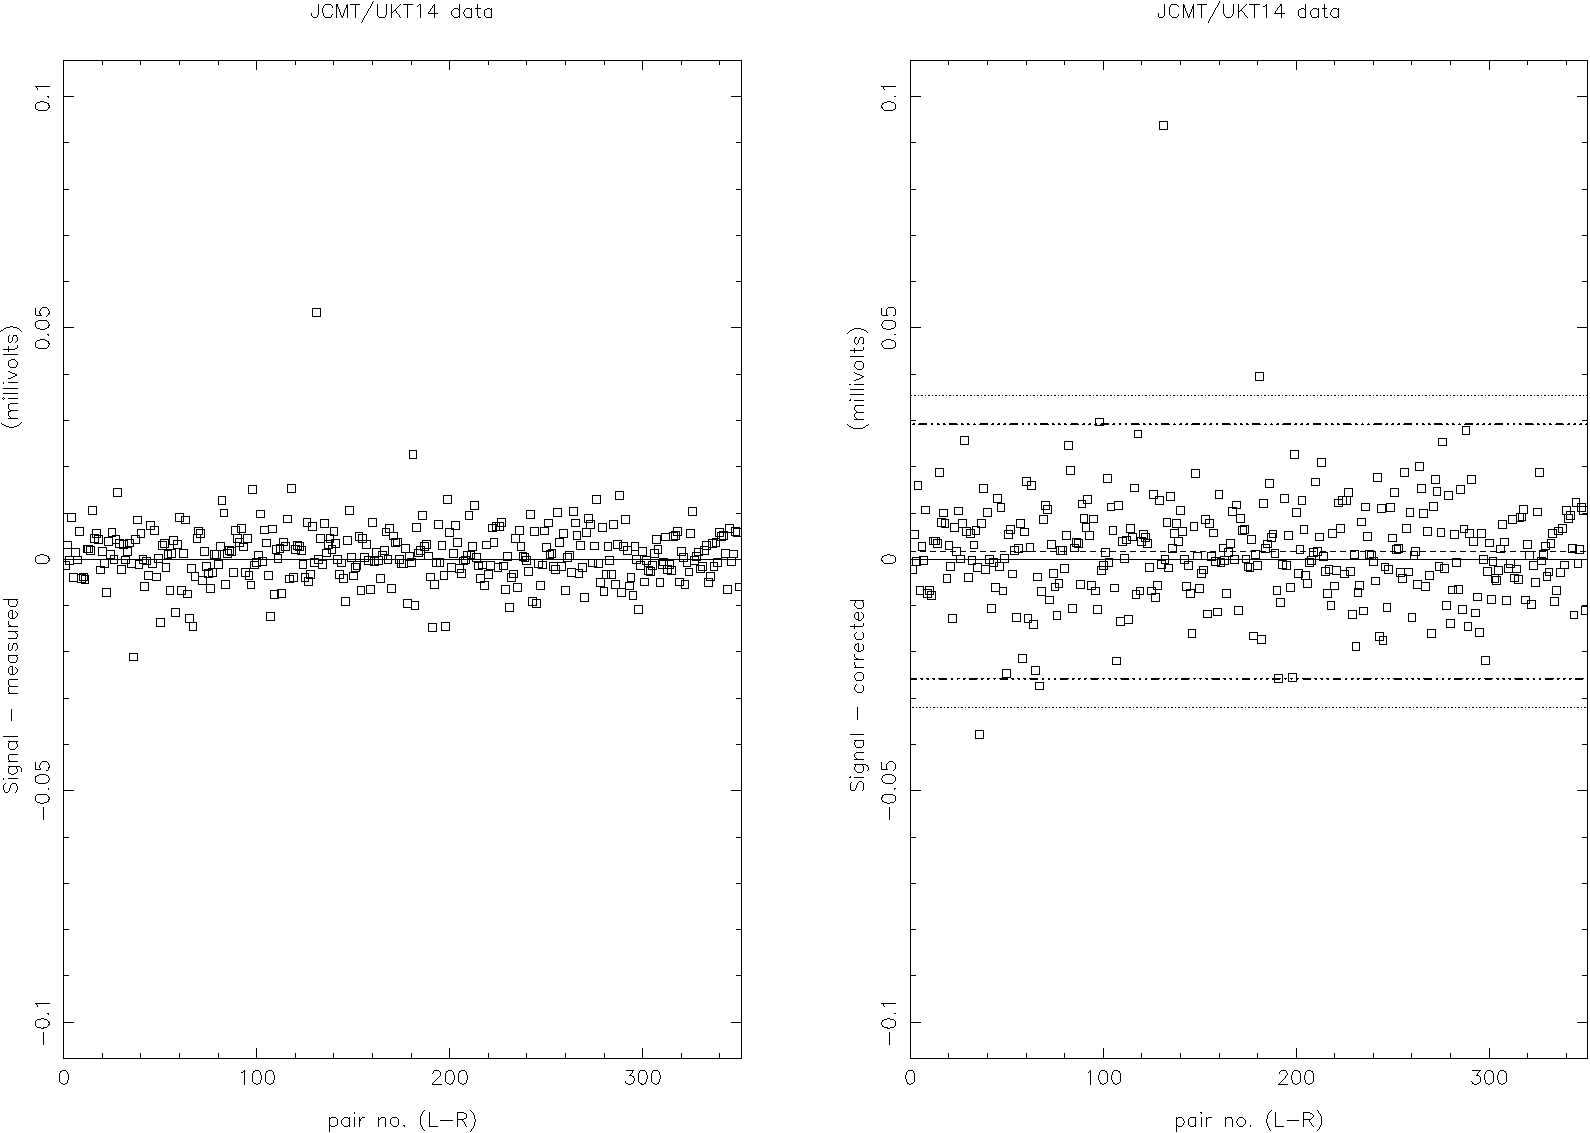
\includegraphics[width=\textwidth]{mtun144fig1}
\caption{
Example plot with our test data.
The left-hand panel shows the raw data (mV) against the running
pair number. The right-hand panel shows the data corrected for
atmospheric extinction. The dashed line indicates the mean value, before
despiking, and the dotted lines represent the 3$\sigma$ deviations from the
mean.}
\label{fig:data}
\end{figure}


The data can be redisplayed showing the data before and after despiking,
demonstrating the success or otherwise of the decision. The
mean, median, standard error and signal-to-noise are again calculated and
displayed.  The mean and median should begin to converge after despiking if
they were previously different.

\noindent{\bf 5.} At this stage the data have been concatenated,
corrected for extinction
and despiked to a satisfactory level. It is now necessary to identify the
periods during which the statistical properties of the data vary significantly
from the rest of the total integration. Such periods should be due to either
short-term fluctuations in opacity, drifting in pointing towards the end of
a long integration or fast changes in telescope focus often encountered if
observing around sunrise or sunset.

The Kolmogorov-Smirnov (hereafter K--S) two sample statistic was used  to test
the null hypothesis that any two independent samples in the data were drawn from
the same parent population. The K--S statistic is simple to calculate and
is sensitive to all types of differences that may exist between the two
population distribution functions making it a powerful test.

The following approach was adopted.
The total coadded integration was chopped up into smaller sub-samples. The user
chooses both the size of the sub-samples and the significance level at which
inconsistent data will be thrown out. Some common-sense has to applied in the
choice of sub-sample size. Examination of the graphical output gives a good
indication of the structure size of any trends in the data.
The first 2 sub-samples are tested against each other and, if passed, are
concatonated. The next sub-sample is then tested against the previously
concatonated data and the procedure repeated, resulting in a continually
increasing statistically consistent sampled observation, until the entire
integration has been tested.

The final mean, median, standard error and signal-to-noise are calculated and
displayed.

An example of the output of the program is given below

\begin{verbatim}

 ... running K-S test to check for statistical consistency
     in the  data. You are asked to choose the size of
     the subsamples (into which the data stream will be
     cut) and the significance level at which pairs will
     be rejected and thrown out from the single scan or
     concatonated data.

 subsample size  : 20

 significance level to reject data : 0.2

 subsample    coadded    total    ifail    statistic    critical level
    20           20       40        0        0.3000        0.3356      passed
    20           40       60        0        0.2000        0.6445      passed
    20           60       60        0        0.3000        0.1214      failed
    20           60       80        0        0.1500        0.8695      passed
    20           80      100        0        0.2250        0.3631      passed
    20          100      100        0        0.2600        0.1874      failed

     MEAN (mV)      MEDIAN       err (mV)     S/N
     0.009587      0.009145      0.001166    8.221

\end{verbatim}

In this example a total of 140 cycles have been split up into 7 subsamples of
20 cycles each. The K--S test is then applied to the first two subsamples
and the test statistic computed. The test statistic is the largest absolute
deviation between the two subsample cumulative distribution functions. In this
particular example the test statistic is 0.3 for the first two subsamples.
The critical level is the probability under the null hypothesis of computing a
value for the test statistic as large as this. In this case the probability
is 0.3356. Since the user has elected to accept any subsample at a probability
greater than 0.2, the two subsamples are combined and the K--S test repeated
for this new combined subsample (40 cycles) together with the next 20 cycles.
The data again passes the K--S test and produces a continuous stream of 60
cycles which is tested against the next 20 cycles. On this occasion the
probability that the data are drawn from the same population is only 0.1214
and since this is $< 0.2$ these 20 cycles are not included.
This procedure is repeated until all the subsamples have been added
in or rejected.

If you wish  to relax the criterion on accepting data then the significance
level, $\alpha$, should be decreased. A value of $\alpha = 0.05$ is often
quoted as the level at which hypotheses are accepted or rejected.

6. After completing the initial pass through the data reduction one can choose
to repeat all or any single part of the process with different parameters
without re-reading the data. Finally the data are calibrated if the
responsivity value (Jy/mV) is known for the filter and aperture of interest.
Your directory is cleaned of the intermediate files that COADD produces.
This is illustrated below.

\begin{verbatim}

 Repeat reduction with these data (Y/N) ? : [N] <cr>

   Calibrate final reduced signal level (mV) via
        known responsivity (Jy/mV)     (Y/N) ? : [N] <cr>


 Summary of reduction in   SUMMARY             .DAT


 ... tidying up .

All versions of the following files will be deleted:

COADD.dat            FOR012.dat  MV.dat
MV_TAUCORRECTED.dat  STDERR.dat  SUMMARY.dat

Is this acceptable? (Y/N) [N] <cr>


\end{verbatim}


A product of the reduction is the calculation of the running standard-error,
$\epsilon $. This should decrease as $\propto n^{-1/2}$, where $n$ is the
number of samples in the concatenated observations which, for equal cycle
times, is a measure of the integration time. In the example shown (Fig.~\ref{fig:error})
5 observations of 50 samples (20
secs/sample) have been concatenated and despiked, producing a total
integration of 5000 seconds
on the quasar Mrk376. The dependence of standard error on integration time,
after despiking,
is clearly very close to the expected $\epsilon \propto t^{-1/2}$, as shown by
the solid line, and demonstrates that even at submillimetre wavelengths, under
reasonable sky conditions, one can continue to improve upper-limits or
the sensitivity of a detection with long integrations.


\begin{figure}[ht]
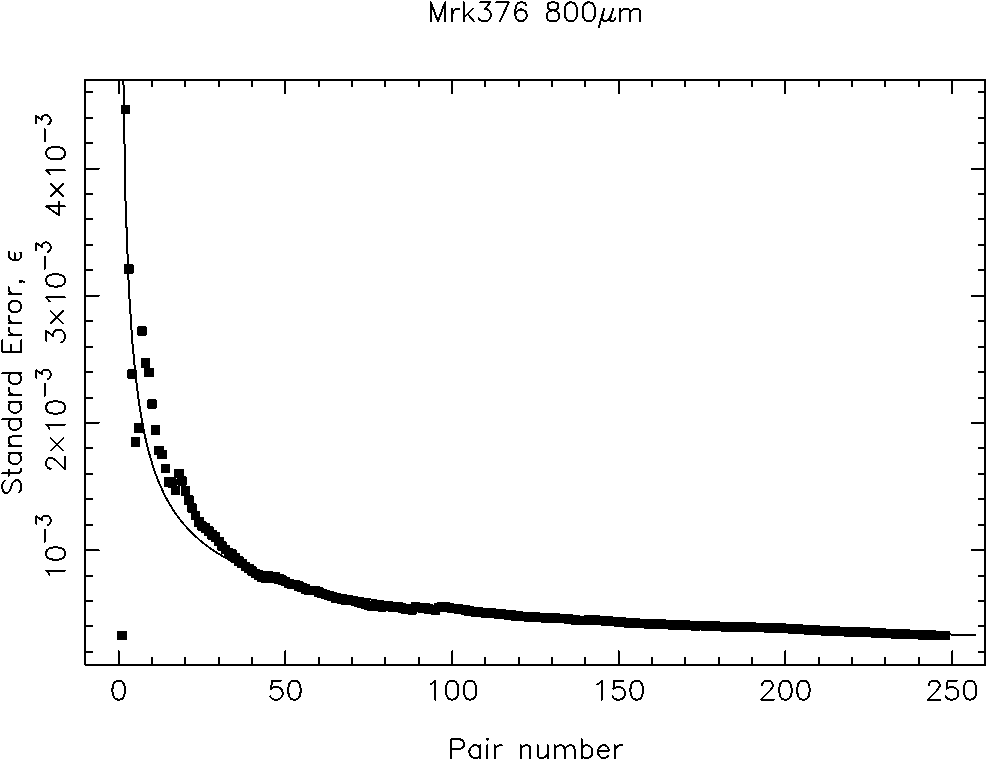
\includegraphics[width=\textwidth]{mtun144fig2}
\caption{
The decrease in standard error, $\epsilon$, for a 5000 second concatenated
integration on Mrk376 is plotted against pair-number (or time for equal
length cycles). The thin line represents $\epsilon \propto t^{-1/2}$ and
demonstrates that the noise properties of the data are close to normal.}
\label{fig:error}
\end{figure}


\end{document}
